\documentclass[
	aspectratio=169, % default is 43
	8pt, % font size, default is 11pt
	%handout, % handout mode without animations, comment out to add animations
]{beamer}
\def\university{}

\documentclass[
	aspectratio=169, % default is 43
	8pt, % font size, default is 11pt
	handout, % handout mode without animations, comment out to add animations
]{beamer}

\usepackage{../template/beamerthemeuulm} % use the inofficial uulm beamer theme
\setfaculty{infIngPsy} % set the color scheme for your faculty here [med/infIngPsy/math/nat]

% requires symbolic links
% git clone git@github.com:SoftVarE-Group/SlideTemplate.git C:\Users\...\SlideTemplate
% mklink /J template C:\Users\...\SlideTemplate
% git clone git@spgit.informatik.uni-ulm.de:thuem/slides.git C:\Users\...\ThomasSlides
% mklink /J thomasslides C:\Users\...\ThomasSlides
\graphicspath{{../template/pics/logos}{../template/pics/nature}{../template/pics/uulm}{../thomasslides/}{../pics/people/}{../pics/xkcd/}}

%\usepackage[ngerman]{babel} % use this line for slides in German
%\recordingtrue % special recording mode for use with a greenscreen, gives you space to show yourself in a layer in front of the slides, has no effect in the handout mode

\title{Software Product Lines} % short title is used for the slide footer but optional

% LINKED LITERATURE

\newcommand{\ludewiglichter}{\href{https://learning.oreilly.com/library/view/-/9781457184932/?ar}{Ludewig and Lichter}}
\newcommand{\seeconomics}{\href{https://rds-ulm.ibs-bw.de/link?kid=027381854}{SE Economics}}
\newcommand{\sommervillelink}[1]{\href{https://ulm.ibs-bw.de/aDISWeb/app?service=direct/0/Home/$DirectLink\&sp=SOPAC00\&sp=SAKSWB-IdNr1615420983}{#1}}
\newcommand{\sommerville}{\sommervillelink{Sommerville}}
\newcommand{\thehumbleprogrammer}{\href{https://dl.acm.org/doi/10.1145/1283920.1283927}{The Humble Programmer}}
\newcommand{\thepragmaticprogrammer}{\href{https://learning.oreilly.com/library/view/the-pragmatic-programmer/9780135956977/}{The Pragmatic Programmer}}

% TYPICAL COMMANDS FOR LECTURES

\renewcommand{\emph}[1]{{\color{blue}\textbf{#1}}}

\newcommand{\deutsch}[1]{{\color{blue}(#1)}}
\newcommand{\deutschertitel}[1]{{\tiny\deutsch{#1}}}

\newcommand{\mycite}[1]{``#1''}
\newcommand{\mytitlesource}[1]{{\tiny\normalfont\mbox{[#1]}}}
\newcommand{\mysource}[1]{\ifthenelse{\equal{#1}{}}{}{\phantom{.}~\hfill~\mytitlesource{#1}}}

\newcommand{\todo}[1]{{\color{red}\textbf{[#1]}}}
\newcommand{\fodo}[1]{\todo{\footnote{\todo{#1}}}}
\newcommand{\todots}{\todo{\ldots}}

% IMPORTED PACKAGES

%\usepackage{adjustbox} % used for partofpage
%\usepackage{tcolorbox} % used for mydefinition, mynote, myexample
\usepackage{multicol} % used temporarily for the lecture overview
\usepackage{mathtools} % required for absolute value in modeling lecture

% COMMANDS TO LAYOUT AND ANNIMATE SLIDES

\newcommand{\lessonslearned}[3]{
	\subsection{Summary}
	\begin{frame}{\insertsection -- \insertsubsection}
		\leftorright{
			\mydefinition{Lessons Learned}{
				\begin{itemize}
					#1
				\end{itemize}
			}
			\mynote{Further Reading}{
				\small % references take space, can be a little smaller
				\begin{itemize}
					#2
				\end{itemize}
			}
		}{
			\myexample{Practice}{
				#3
			}
		}
	\end{frame}
}

% TODO temporary hack to layout the slide overview in two colums
\renewcommand{\lectureoverview}{
%	\section*{Overview}
%	\subsection*{Overview}
	\begin{frame}{\insertsubtitle}
		\begin{multicols}{2}
			\tableofcontents
		\end{multicols}
	\end{frame}
}

\renewcommandx{\maketitle}[2][1=apr21-o25a,2=150]{
    {
	\usebackgroundtemplate{} % TODO temporary hack to enable missing pictures at title slide
	%\ifx {#1} \empty \else {\usebackgroundtemplate{\includegraphics[trim=0 0 0 #2,clip,width=\paperwidth]{#1}}} \fi     
	%\usebackgroundtemplate{\includegraphics[trim=0 0 0 #2,clip,width=\paperwidth]{#1}}
    \begin{frame}[plain]
        \vskip0pt plus 1filll
        \begin{beamercolorbox}[wd=\paperwidth,ht=4.5ex,dp=2ex,right]{titlebox}
            \LARGE\textbf{\inserttitle}\hspace*{20pt}
        \end{beamercolorbox}%
        \nointerlineskip%
        \begin{beamercolorbox}[wd=\paperwidth,ht=2.25ex,dp=1ex,right]{subtitlebox}
            \small 
            \ifx \insertsubtitle \empty \else \insertsubtitle\ $\vert$ \fi
            \insertauthor\
            \ifx \insertdate \empty \else $\vert$ \insertdate \fi
            \hspace*{20pt}
        \end{beamercolorbox}%
        \nointerlineskip%
        \begin{beamercolorbox}[wd=\paperwidth,ht=4.5ex,dp=2ex,left]{logobox}
            \centering
            \vspace{-1ex}
            \hspace{10pt}
            \includegraphics[height=4.5ex]{sp} % SPECIFY INSTITUTE LOGO HERE
            \hfill
            \includegraphics[height=4.5ex]{uulm}
            \hspace{10pt}
        \end{beamercolorbox}%
    \end{frame}
    }  
}

%
%\newcommand{\onlyleft}[1]{
%	\halfpage{#1}
%}
%
%\newcommand{\onlyright}[1]{
%	~\hfill
%	\halfpage{#1}
%}
%
%\newcommand{\leftorright}[2]{
%	\uncover<1>{\halfpage{#1}}
%	\hfill
%	\uncover<3->{\halfpage{#2}}
%}
%
%\newcommand{\rightorleft}[2]{
%	\uncover<3->{\halfpage{#1}}
%	\hfill
%	\uncover<1>{\halfpage{#2}}
%}
%
%\newcommand{\leftthenright}[2]{
%	\halfpage{#1}
%	\hfill\pause
%	\halfpage{#2}
%}
%
%\newcommand{\leftandright}[2]{
%	\halfpage{#1}
%	\hfill
%	\halfpage{#2}
%}
%
%\newcommand{\leftmiddleandright}[3]{
%	\thirdpage{#1}
%	\hfill
%	\thirdpage{#2}
%	\hfill
%	\thirdpage{#3}
%}
%
%\newcommand{\leftmiddleorright}[3]{
%	\uncover<1>{\thirdpage{#1}}
%	\hfill
%	\uncover<3>{\thirdpage{#2}}
%	\hfill
%	\uncover<5->{\thirdpage{#3}}
%}
%
%\newcommand{\halfpage}[1]{\partofpage{48}{#1}}
%
%\newcommand{\thirdpage}[1]{\partofpage{31}{#1}}
%
%\newcommand{\partofpage}[2]{
%	\adjustbox{valign=t}{\begin{minipage}{0.#1\textwidth}
%			\begin{flushleft}
%				#2
%			\end{flushleft}
%	\end{minipage}}
%}
%
%\newcommand{\mydefinition}[2]{
%	\begin{tcolorbox}[title=#1,colback=orange!10,colframe=orange!30,coltitle=black,fonttitle=\bfseries,left=1mm,right=1mm,top=1mm,bottom=1mm]
%		\begin{flushleft}
%			#2
%		\end{flushleft}
%	\end{tcolorbox}
%}
%
%\newcommand{\mydefinitiontight}[2]{
%	\begin{tcolorbox}[title=#1,colback=white,colframe=orange!30,coltitle=black,fonttitle=\bfseries,left=0mm,right=0mm,top=0mm,bottom=0mm]
%		\begin{flushleft}
%			#2
%		\end{flushleft}
%	\end{tcolorbox}
%}
%
%\newcommand{\mynote}[2]{
%	\begin{tcolorbox}[title=#1,colback=red!10,colframe=red!30,coltitle=black,fonttitle=\bfseries,left=1mm,right=1mm,top=1mm,bottom=1mm]
%		\begin{flushleft}
%			#2
%		\end{flushleft}
%	\end{tcolorbox}
%}
%
%\newcommand{\myexample}[2]{
%	\begin{tcolorbox}[title=#1,colback=blue!10,colframe=blue!30,coltitle=black,fonttitle=\bfseries,left=1mm,right=1mm,top=1mm,bottom=1mm]
%		\begin{flushleft}
%			#2
%		\end{flushleft}
%	\end{tcolorbox}
%}
%
%\newcommand{\myexampletight}[2]{
%	\begin{tcolorbox}[title=#1,colback=white,colframe=blue!30,coltitle=black,fonttitle=\bfseries,left=0mm,right=0mm,top=0mm,bottom=0mm]
%		\begin{flushleft}
%			#2
%		\end{flushleft}
%	\end{tcolorbox}
%}

\subtitle{8. Development Process}
\author{Thomas Thüm, Elias Kuiter, Timo Kehrer}

\begin{document}

\mode<handout>{\contentoverview}

\mode<beamer>{
	\ifdefined\thepicture
		\maketitle[\thepicture][\thepictureoffset]
	\else
		\maketitle[]
	\fi
}

% shared slide content

% introduced: 02a-configuration
% reused: 03a-intro
\newcommand{\frameImplementSPLs}{
	\begin{mycolumns}[widths={45},animation=none]
		\pic[width=\linewidth]{metaproduct2}
	\mynextcolumn
		\begin{note}{Key Issues}
			\begin{itemize}
			\item Systematic reuse of implementation artifacts
			\item Explicit handling of variability
			\end{itemize}
		\end{note}
		\uncover<2->{\begin{definition}{Variability\mysource{\fospl\mypage{48}}}
			\mycite{\emph{Variability} is the ability to derive different products from a common set of artifacts.}
		\end{definition}}
		~
		\uncover<3->{\begin{note}{Variability-Intensive System}
			Any software product line is a variability-intensive system. % TODO Timo: do we really need this term? where does this definition come from?
		\end{note}}
	\end{mycolumns}
}

% introduced: 02a-configuration
% reused: 02b-implementation, 03a-intro
\newcommand{\frameVariabilityAndBindingTimes}{
	\begin{mycolumns}[widths={55},animation=none]
		\begin{definition}{Binding Time \deutsch{Bindungszeitpunkt}\mysource{\fospl\mypage{48}}}
			\begin{itemize}
				\item Variability offers choices
				\item Derivation of a product requires to make decisions (aka. binding)
				\item Decisions may be bound at different binding times
			\end{itemize}
		\end{definition}
		~
		\uncover<2->{\begin{note}{When? By whom? How?}
			\lectureruntime\parta: \emph{when} and \emph{by whom}

			\lectureruntime\partb: \emph{how}
		\end{note}}
	\mynextcolumn
		\pic[width=\linewidth]{metaproduct2}
	\end{mycolumns}
}

% introduced: 03a-intro
% reused: 03a-intro
\newcommand{\frameRuntimeVariabilityProblems}{
	\begin{note}{Problems of Runtime Variability}
		{\bf Conditional Statements:}
		\begin{itemize}
			\item Code scattering, tangling, and replication
		\end{itemize}
		{\bf Design Patterns for Variability:}
		\begin{itemize}
			\item Trade-offs and potential negative side effects
			\item Constraints that may restrict their usage
		\end{itemize}
		{\bf In General:}
		\begin{itemize}
			\item Variable parts are always delivered
			\item Not well-suited for compile-time binding
		\end{itemize}
	\end{note}
}

% introduced: 03a-intro
% reused: 03a-intro
\newcommand{\frameSoftwareConfigurationManagement}{
	\begin{mycolumns}
		\begin{definition}{Software Configuration Management} % TODO source missing
			Policies, processes, and tools for managing evolving software systems:
			\begin{itemize}
				\item Version control
				\item System building
				\item Release management
				\item Change management
				\item Collaborative work
			\end{itemize}
		\end{definition}
	\mynextcolumn
		\begin{note}{No Software Configuration Management}
			\lecturecloneandown\parta: Ad-Hoc Clone-and-Own

			aka.\ unmanaged clone-and-own
		\end{note}
		\begin{note}{Version Control}
			\lecturecloneandown\partb: Clone-and-Own with Version Control

			instance of managed clone-and-own
		\end{note}
		\begin{note}{System Building}
			\lecturecloneandown\partc: Clone-and-Own with Build Systems

			instance of managed clone-and-own
		\end{note}
	\end{mycolumns}
}


\section{Domain and Application Engineering}

% TODO would be good to refer to existing implementation techniques more explicitly in this part

\subsection{Recap: Process Models}
\begin{frame}{\inserttitle}
	\lectureseriesoverview[8]
\end{frame}

\begin{frame}{\myframetitle\ \deutschertitel{Vorgehensmodelle}}
	\begin{definition}{Recap: The Software Life Cycle\ \deutschertitel{Der Softwarelebenszyklus}}
		\renewcommand{\projectcartoonwidth}{.17}
		\waterfallcartoon
	\end{definition}
	\begin{mycolumns}[animation=none]
		\uncover<2->{\begin{example}{Process Models for Single-System Engineering}
			waterfall model, V model, scrum, \ldots
		\end{example}}
	\mynextcolumn
		\uncover<3->{\begin{note}{Process Models for Product-Line Engineering}
			???
		\end{note}}
	\end{mycolumns}
\end{frame}

\begin{frame}{Recap: Domain}
	\begin{mycolumns}[animation=none]
		\begin{definition}{Recap: Domain \deutsch{Domäne} \hfill\mysource{\lectureintroduction}}
			\mycitebegin A \emph{domain} is an area of knowledge that:
			\begin{itemize}
				\item is scoped to maximize the satisfaction of the requirements of its stakeholders,
				\item includes a set of concepts and terminology understood by practitioners in that area,
				\item and includes the knowledge of how to build software systems (or parts of
				software systems) in that area.\myciteend
			\end{itemize}
		\end{definition}
	\mynextcolumn
	\end{mycolumns}
\end{frame}
% TODO introduce domain and application artifacts here? see \sple
% would also apply to domain/application requirements, but domain requirement is a confusing term (as it would refer to requirements of a product line and not all of a domain)

\subsection{Domain and Application Engineering}
\begin{frame}{\myframetitle}
	\begin{note}{A Process Model for Product-Line Engineering}
		idea: split development into two phases, one for product line and one for products
	\end{note}
	\begin{mycolumns}[animation=none,T]
		\uncover<2->{\begin{definition}{Domain Engineering\mysource{\fospl\mypages{21--22}}}
			\mycite{\emph{Domain engineering} is the process of analyzing the domain of a product line and developing reusable artifacts.}
		\end{definition}
		\begin{note}{Domain Engineering\mysource{\fospl\mypage{21}}}
			\begin{itemize}
				\item development for reuse
				\item prepares artifacts to be used in products (or during application engineering)
				\item goal: reduce effort per product (i.e., effort during application engineering)
			\end{itemize}
		\end{note}}
	\mynextcolumn
		\uncover<3->{\begin{definition}{Application Engineering\mysource{\fospl\mypage{21}}}
			\mycite{\emph{Application engineering} has the goal of developing a specific product for the needs of a particular customer (or other stakeholder).}
		\end{definition}
		\begin{note}{Application Engineering\mysource{\fospl\mypage{21}}}
			\begin{itemize}
				\item development with reuse
				\item build products using artifacts from domain engineering
				\item repeated for every product
				\item \mycite{application} of the product line (i.e., suitable for application and system software)
			\end{itemize}
		\end{note}}
	\end{mycolumns}
\end{frame}

% terms used in the remainder are mostly taken from \sple and some from \fospl
\begin{frame}[label=DomainAndApplicationEngineeringDiagram]
	\footnotesize%
	\begin{mycolumns}[columns=3,widths={10,70,10},animation=none]
		\renewcommand{\projectcartoonwidth}{1}\projectcartoon{01}{Product-Line Requirements}
	\mynextcolumn
		\begin{note}{Domain Engineering}
			\renewcommand{\projectcartoonwidth}{.15}%
			\projectcartoon{02}{Domain Analysis}%
			\projectcartoon{03}{Domain Design}%
			\projectcartoon{04}{Domain Implementation}%
			\projectcartoon{05}{Domain Testing}
		\end{note}
	\mynextcolumn
	\end{mycolumns}
	\pause
	\begin{mycolumns}[columns=3,widths={10,70,10},animation=none]
		\renewcommand{\projectcartoonwidth}{1}\hprojectcartoon{01}{Product Requirements}
	\mynextcolumn
		\begin{note}{Application Engineering}
			\renewcommand{\projectcartoonwidth}{.15}%
			\hprojectcartoon{02}{Application Analysis}%
			\hprojectcartoon{03}{Application Design}%
			\hprojectcartoon{04}{Application Implementation}%
			\hprojectcartoon{05}{Application Testing}
		\end{note}
	\mynextcolumn
		\renewcommand{\projectcartoonwidth}{1}\hprojectcartoon{13}{Product}
	\end{mycolumns}
\end{frame}

\subsection{Analysis and Design}
\begin{frame}{Domain and Application Analysis}\small
	\begin{mycolumns}[T,columns=3,widths={10}]
		\renewcommand{\projectcartoonwidth}{1}\hprojectcartoon{02}{}
	\mynextcolumn
		\begin{definition}{Domain Analysis\mysource{\fospl\mypage{21}, \sple\mypage{25}}}
			\begin{itemize}
				\item requirements analysis for a product line
				\item define scope of the product line
				\item which features are in scope?
				\item which combinations of features are in scope?
				\item typically results in a feature model and features mapped to requirements
			\end{itemize}
		\end{definition}
		\begin{definition}{Domain Scoping\mysource{\fospl\mypage{22}}}
			which requirements of a domain are in scope for the product line?
			\begin{itemize}
				\item domain experts collect requirements (e.g., from existing systems, interviews, potential customers)
				\item often economical decision by managers
			\end{itemize}
		\end{definition}
		% TODO introduce term Domain Modeling?
	\mynextcolumn
		\begin{definition}{Application Analysis\mysource{\fospl\mypages{21--25}}}
			\begin{itemize}
				\item requirements analysis for a product
				\item based on the output of domain analysis
				\item ideally: customer requirements mapped to a feature selection
				\item alternative strategies for new and unsupported requirements:
					\begin{enumerate}\small % TODO Benno: why is the font size changed here?
						\item requirement is out of scope (i.e., no product made available)
						\item document for custom development (i.e., development in application engineering)
						\item integrate into domain analysis (i.e., development in domain engineering)
					\end{enumerate}
				\item best strategy depends on the situation
			\end{itemize}
		\end{definition}
		% TODO pointer to staged configuration? or even introduce it here?
	\end{mycolumns}
\end{frame}
% TODO running example

\begin{frame}{Domain Scoping in Practice}
	\begin{mycolumns}[widths={70},animation=none]
		\centering\pic[width=\linewidth]{toyota-aygo-mirrorcovers}
	\mynextcolumn
		\begin{example}{Aygo Mirror Covers}
			Can customers choose \ldots
			\begin{itemize}
				\item mirror covers? Yes!
				\item different covers for left and right side? Yes!
				\item multiple covers for the same side? Yes!
				\item between 2, 3, 4, \ldots\ colors and which ones?
			\end{itemize}
		\end{example}
	\end{mycolumns}
\end{frame}

\begin{frame}{Domain Scoping in Practice}
	\begin{mycolumns}[widths={70},animation=none]
		\centering\picDark[width=\linewidth]{linux-architectures}
	\mynextcolumn
		\begin{example}{Linux Kernel Architectures}
			\begin{itemize}
				\item in Linux, $\approx 20$ CPU architectures are carefully maintained in 2023
				\item to keep it manageable, obsolete architectures are regurlarly removed
				\item requires an answer to ``is this architecture still used by a relevant number of people?''
			\end{itemize}
		\end{example}
	\end{mycolumns}
\end{frame}

\begin{frame}{Domain and Application Design}
	\begin{mycolumns}[T,columns=3,widths={10,50}]
		\renewcommand{\projectcartoonwidth}{1}\hprojectcartoon{03}{}
	\mynextcolumn
		\begin{definition}{Domain Design\mysource{\sple\mypage{26}}} % TODO see \sple Chapter 6+11
			\begin{itemize}
				\item development of a reference architecture (e.g., client-server or pipe-and-filter)
				\item common, high-level structure for all products
				\item decision on implementation technique
					\begin{itemize}
						\item runtime variability: (immutable) global variables, method parameters
						\item clone-and-own: ad-hoc, with version control, with build systems
						\item conditional compilation: build systems, preprocessors
						\item modular features: components, services, frameworks with plug-ins
						\item modularization of crosscutting concerns: feature-oriented, aspect-oriented programming
						\item combinations thereof
					\end{itemize}
			\end{itemize}
		\end{definition}
	\mynextcolumn
		\begin{definition}{Application Design\\\mysource{\sple\mypages{32--33}}}
			\begin{itemize}
				\item create application architecture
				\item derived from reference architecture
				\item based on feature selection
				\item design decisions for application-specific requirements
			\end{itemize}
		\end{definition}
	\end{mycolumns}
\end{frame}

\subsection{Implementation and Testing}
\begin{frame}{Domain and Application Implementation}
	\begin{mycolumns}[T,columns=3,widths={10}]
		\renewcommand{\projectcartoonwidth}{1}\hprojectcartoon{04}{}
	\mynextcolumn
		\begin{definition}{Domain Implementation\mysource{\fospl\mypage{21}}} % TODO see \sple Chapter 7+12
			\begin{itemize}
				\item development of reusable artifacts
				\item implementation of features identified during domain analysis
				\item implementation largely depends on the implementation technique chosen in domain design
			\end{itemize}
		\end{definition}
	\mynextcolumn
		\begin{definition}{Application Implementation\mysource{\fospl\mypage{21}}}
			\begin{itemize}
				\item development of products based on reusable artifacts
				\item ideally: fully automated generation (aka.\ \emph{product derivation})
				\item full automation not feasible \ldots
					\begin{enumerate}
						\item when custom development is needed (i.e., for application-specific requirements)
						\item for clone-and-own, components, services
					\end{enumerate}
			\end{itemize}
		\end{definition}
	\end{mycolumns}
\end{frame}
% reusable parts indespensible, reusable architecture optional
% fully automatic or semi-automatic with custom design and implementation

\begin{frame}{Domain and Application Testing}
	\begin{mycolumns}[T,columns=3,widths={10}]
		\renewcommand{\projectcartoonwidth}{1}\hprojectcartoon{05}{}
	\mynextcolumn
		\begin{definition}{Domain Testing\mysource{\sple\mypage{27}}} % TODO see \sple Chapter 8+13
			\begin{itemize}
				\item validation and verification of reusable artifacts
				\item development of reusable tests
				\item testing of features in isolation, if possible\mysource{more in \lectureanalyses}
				\item testing of sample products\\\mysource{more in \lecturetesting}
			\end{itemize}
		\end{definition}
	\mynextcolumn
		\begin{definition}{Application Testing\mysource{\sple\mypages{33--34}}}
			\begin{itemize}
				\item testing of the application
				\item reuse of test artifacts from domain testing
				\item new test artifacts for custom development
			\end{itemize}
		\end{definition}
	\end{mycolumns}
\end{frame}
% systematic testing, sometimes skipped (e.g., if product derivation not automatic)
% testing of a single product, sometimes optional

\subsection{Overview on Domain and Application Engineering}
\againframe{DomainAndApplicationEngineeringDiagram}

\subsection{Problem and Solution Space}
\begin{frame}{\myframetitle}
	\begin{mycolumns}[widths={35},T]
		\begin{definition}{Problem Space\mysource{\fospl\mypage{21}}}
			\mycite{The \emph{problem space} takes the perspective of stakeholders and their problems, requirements, and views of the entire domain and individual products. Features are, in fact, domain abstractions that characterize the problem space.}\\\mysource{\lecturemodeling}
		\end{definition}
		{\small\featureDiagram{Graph,abstract[Directed,optional,concrete][Weighted,optional,concrete][OptimalConnection,optional,concrete]}}
		
		\centering
		\pic[width=.4\linewidth]{preprocessor-wilderness-problem-space}
	\mynextcolumn
		\begin{definition}{Solution Space\mysource{\fospl\mypage{21}}}
			\mycite{The \emph{solution space} represents the developer’s and vendor’s perspectives. It is characterized by the terminology of the developer, which includes names of functions, classes, and program parameters. The solution space covers the design, implementation, and validation and verification of features and their combinations in suitable ways to facilitate systematic reuse.}\\\mysource{\lectureruntime, \lecturecloneandown, \lecturefeatures, \lecturemodules, \lecturelanguages}
		\end{definition}
		\centering
		\pic[width=.6\linewidth,trim=20 20 20 40,clip]{preprocessor-wilderness-solution-space}
	\end{mycolumns}
\end{frame}

% TODO lecture 8: show how linux in lecture 4+5 relates to problem space (kconfig)/mapping (kbuild)/solution space (cpp) - put this into the four-quadrant model

% TODO visual summary, including pictures from earlier lectures and references to lectures - not sure whether more content fits into this part

\lessonslearned{
	\item \ldots
}{
	\item \ldots
}{
	\ldots
}

\sectionend

\section{Product-Line Implementation}

\subsection{Recap: Runtime Variability}

\begin{frame}[fragile]{\myframetitle}
	\footnotesize
	\begin{mycolumns}[animation=none]
\begin{codetight}{}
public class Config {
	~public static boolean COLORED = true;~
	@public static boolean WEIGHTED = false;@
}
\end{codetight}
\begin{codetight}{}
public class Graph {
	...
	Edge add(Node n, Node m) {
		Edge e = new Edge(n, m);
		nodes.add(n); nodes.add(m); edges.add(e);
		@if (Config.WEIGHTED) { e.weight = new Weight(); }@
		return e;
	}
	@Edge add(Node n, Node m, Weight w) {
		if (!Config.WEIGHTED) { throw new RuntimeException(); }
		Edge e = new Edge(n, m);
		nodes.add(n); nodes.add(m); edges.add(e);
		e.weight = w;
		return e;
	}@
	...
}
\end{codetight}
	\mynextcolumn
\begin{codetight}{}
public class Node {
	~Color color;~
	...
	Node(){
		~if (Config.COLORED) { color = new Color(); }~
	}
	void print() {
		~if (Config.COLORED) { Color.setDisplayColor(color); }~
		System.out.print(id);
	}
}
\end{codetight}
\begin{codetight}{}
public class Edge {
	@Weight weight;@
	...
	Edge(Node _a, Node _b) {
		a = _a; b = _b;
		@if (Config.WEIGHTED) { weight = new Weight(); }@
	}
	void print() {
		a.print(); b.print();
		@if (Config.WEIGHTED) { weight.print(); }@
	}
}
\end{codetight}
	\end{mycolumns}
\end{frame}

\begin{frame}{\myframetitle}
	\begin{mycolumns}[widths={40},T]
		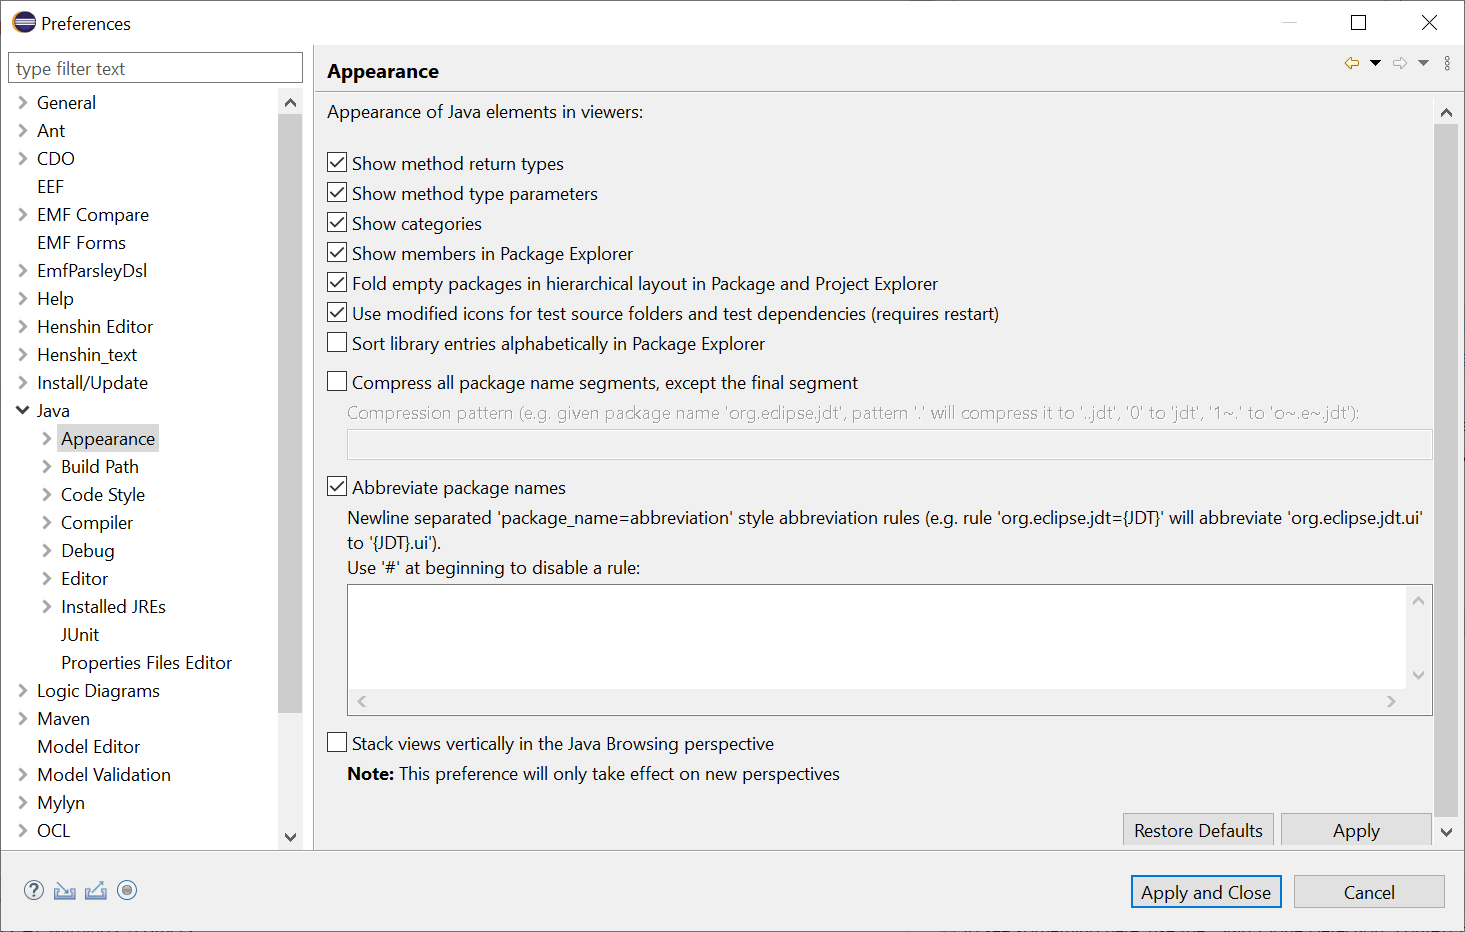
\includegraphics[width=\linewidth]{preferences-eclipse}

		\begin{definition}{How to? -- Preference Dialog}
			\begin{itemize}
				\item implement runtime variability
				\item compile the program
				\item manually adjust preferences based on configuration
				\item run the program
			\end{itemize}
		\end{definition}
	\mynextcolumn
		\leftandright{
			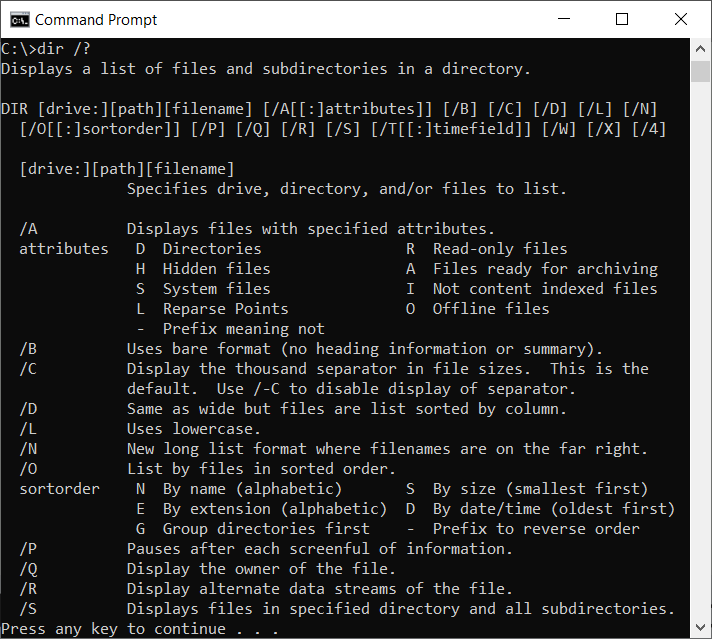
\includegraphics[width=\linewidth]{runtime-parameters-win10-cmd-dir}
		}{
			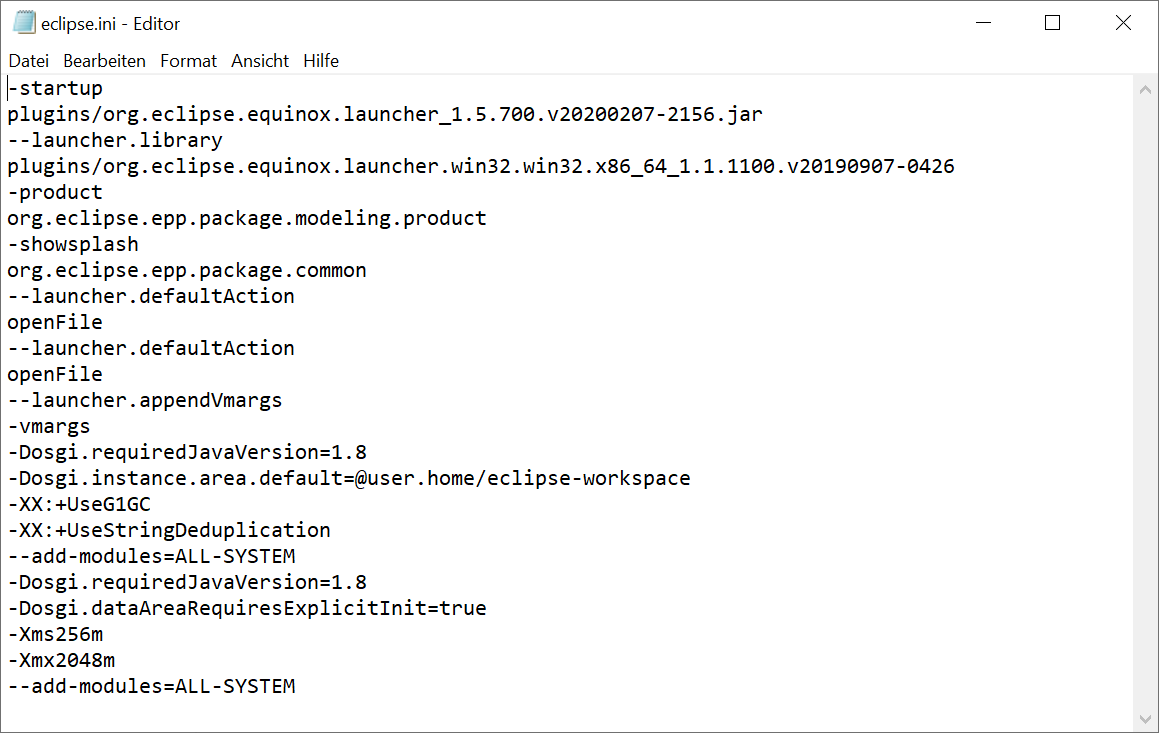
\includegraphics[width=\linewidth]{configfile-eclipse-ini}
		}

		\begin{definition}{How to? -- Command-Line Options / Configuration Files}
			\begin{itemize}
				\item implement runtime variability
				\item compile the program
				\item automatically generate command-line options / configuration files based on configuration
				\item run the program
			\end{itemize}
		\end{definition}
	\end{mycolumns}
\end{frame}

\begin{frame}[fragile]{\myframetitle}
	\begin{mycolumns}[widths={48}]
\begin{codetight}[basicstyle=\small]{}
public class Config {
	~public final static boolean COLORED = true;~
	@public final static boolean WEIGHTED = false;@
}
\end{codetight}
		\begin{definition}{How to? -- Immutable Global Variables}
			\begin{itemize}
				\item implement runtime variability
				\item automatically generate class with global variables based on configuration
				\item compile and run the program
			\end{itemize}
		\end{definition}
	\mynextcolumn
		\begin{note}{What is missing?}
			\begin{itemize}
				\item automated generation:\\\hfill for preference dialogs
				\item no compile-time variability / same large binary:\\\hfill for all except immutable global variables
				\item very limited compile-time variability:\\\hfill for immutable global variables
			\end{itemize}
		\end{note}
		\mynote{Other Problems}{
			{\bf Conditional Statements:}
			\begin{itemize}
				\item Code scattering, tangling, and replication.
			\end{itemize}	
			{\bf Design Patterns for Variability:}
			\begin{itemize}
				\item Trade-offs and potential negative side effects.
				\item Constraints that may restrict their usage.
			\end{itemize}
		}	
	\end{mycolumns}
\end{frame}

\subsection{Recap: Clone-and-Own}

\begin{frame}{\myframetitle}
	\begin{mycolumns}[columns=2,widths={50,50},animation=none]
		\mydefinition{Clone-and-Own}{
			\begin{itemize}
				\item New variants of a software system are created by copying and adapting an existing variant.
				\item Afterwards, cloned variants evolve independently of each other.
			\end{itemize}	
		}	
		\vspace{3mm}		
		\myexample{Cloning Whole Products (Clone-and-Own)}{~\hfill
\includegraphics[width=.2\linewidth]{130}\hfill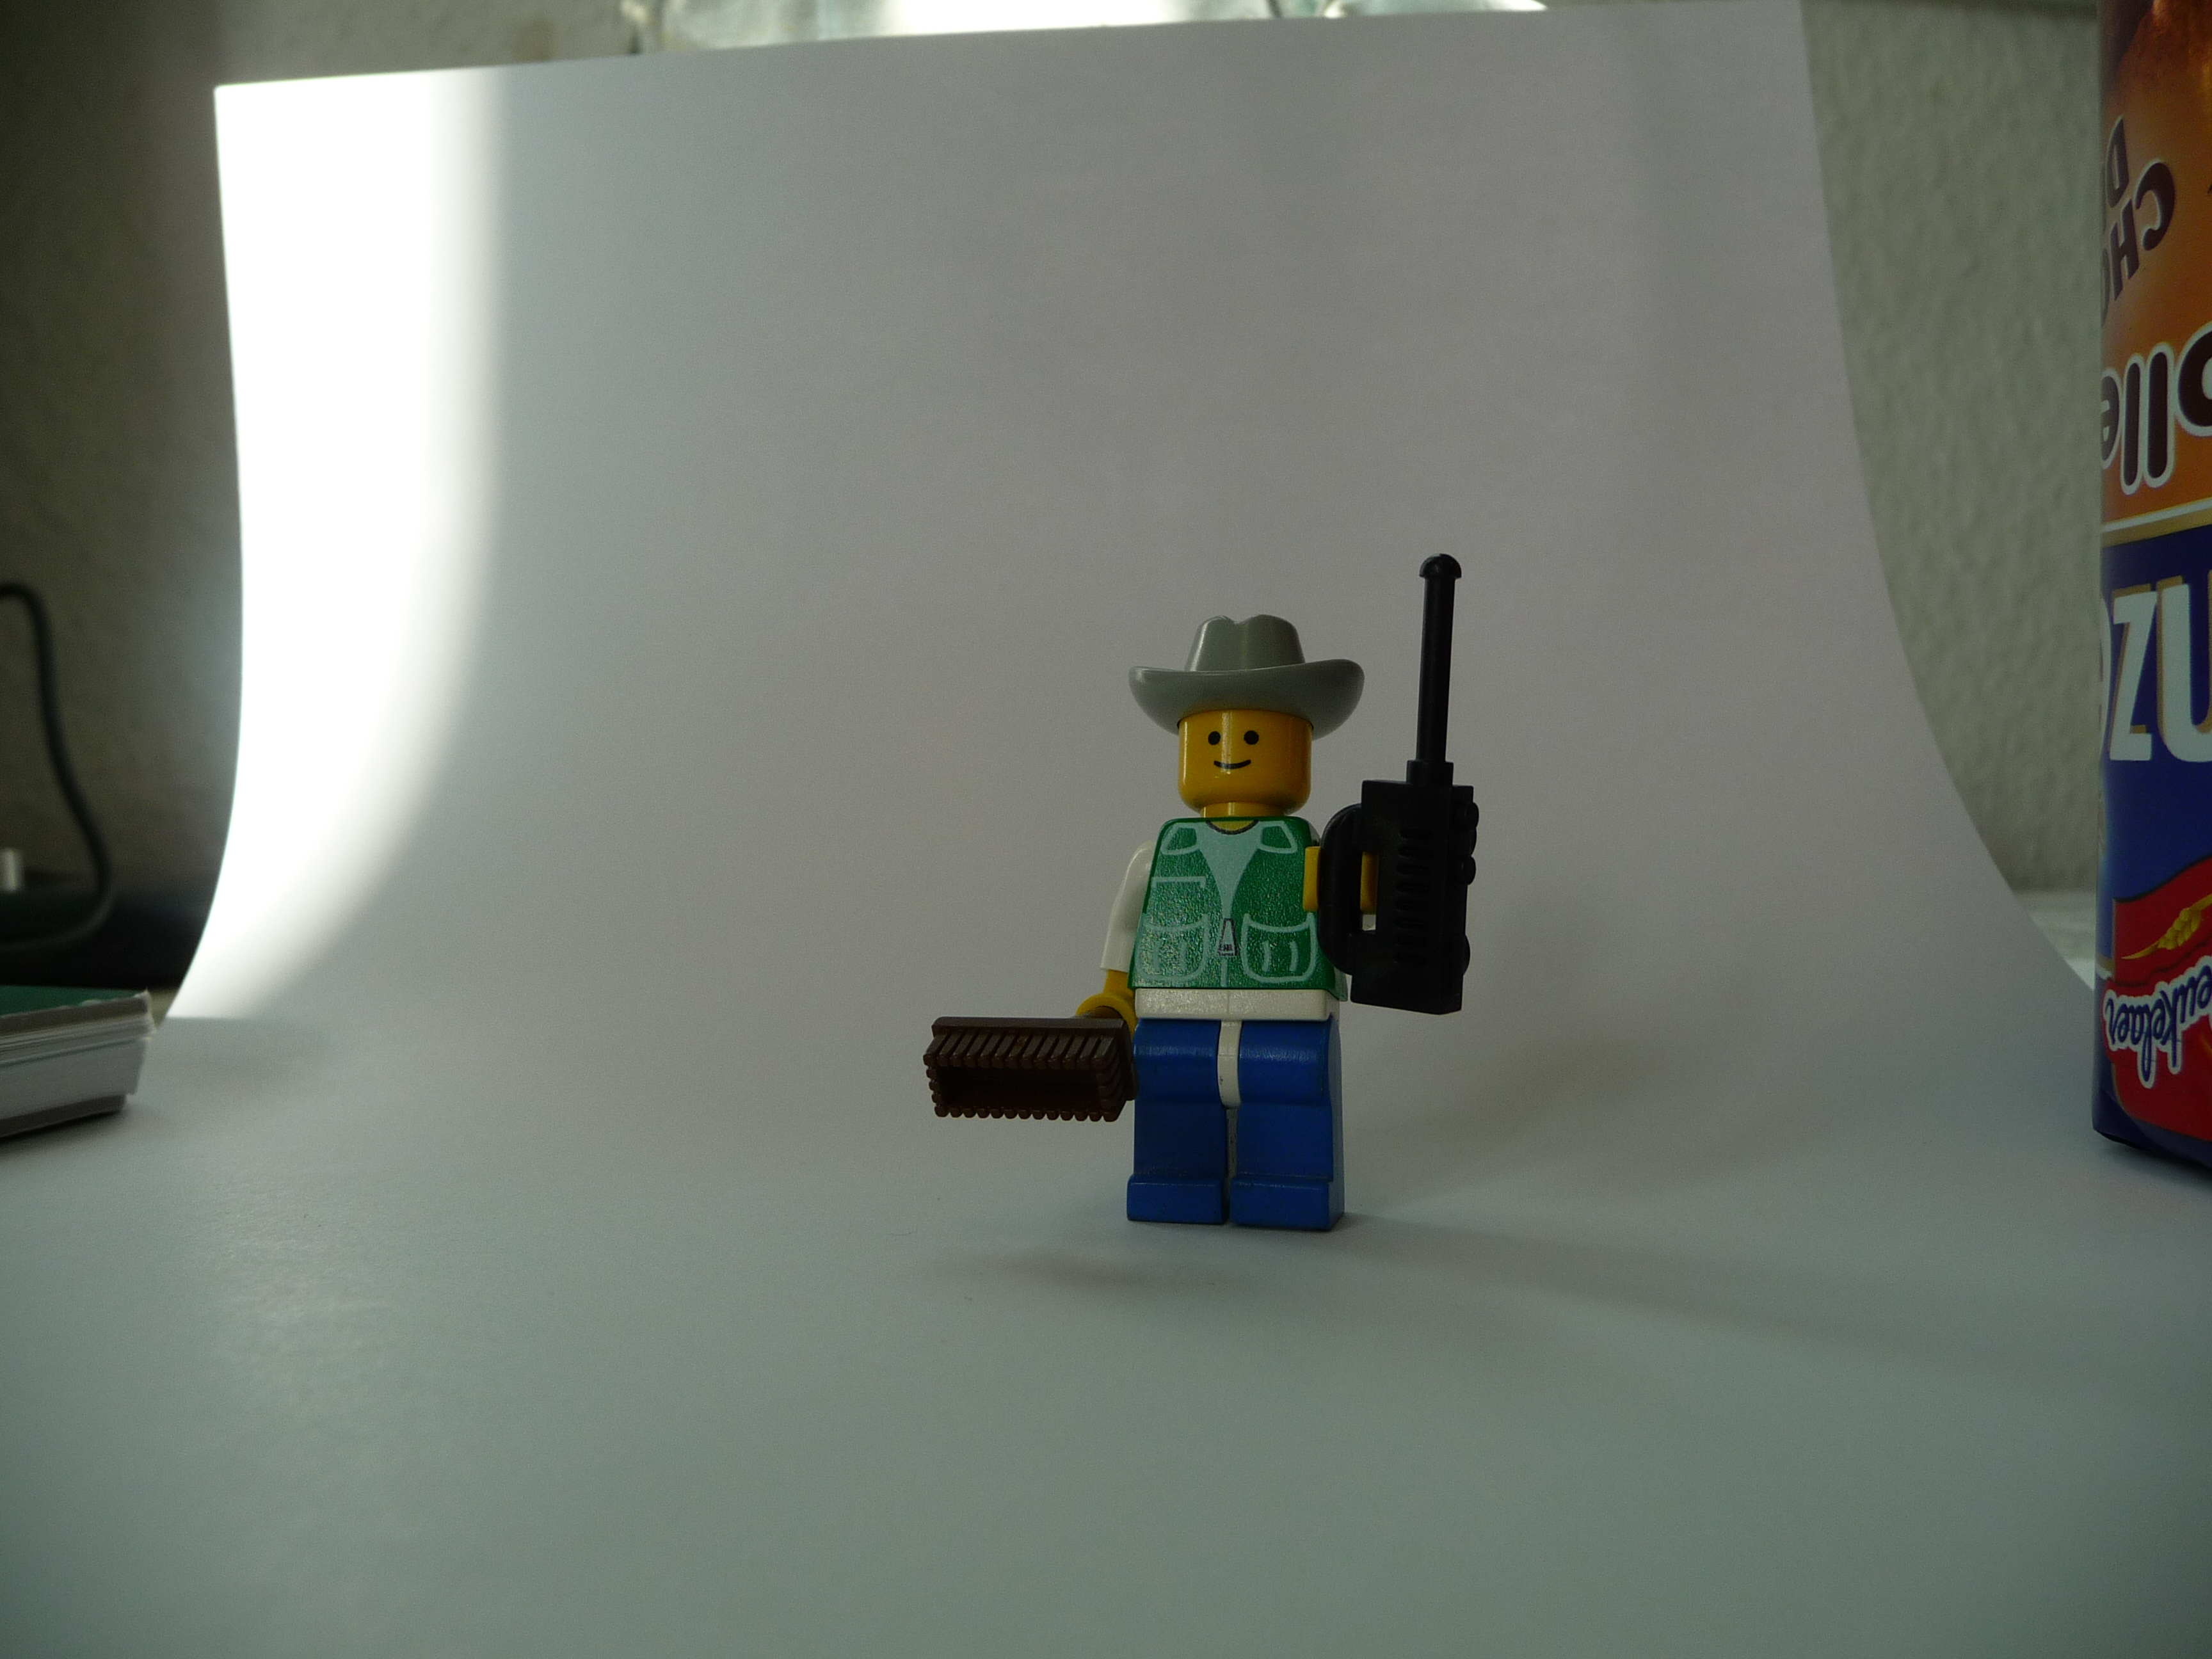
\includegraphics[width=.2\linewidth]{230}\hfill~}
	\mynextcolumn
		\pic[width=\linewidth,page=24]{lego}
	\end{mycolumns}
\end{frame}

\begin{frame}{\myframetitle}
	\begin{mycolumns}[widths={30}]
		\centering~

		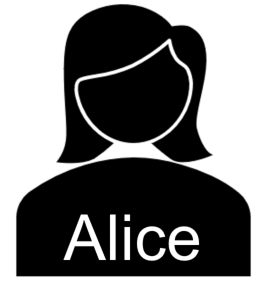
\includegraphics[scale=0.2]{alice}
		\includegraphics[scale=0.26,page=2]{graphs}

		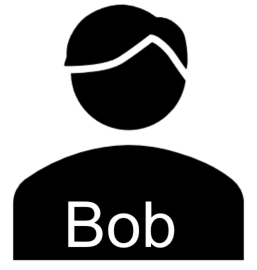
\includegraphics[scale=0.2]{bob}
		\includegraphics[scale=0.26,page=12]{graphs}

		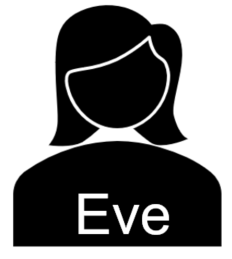
\includegraphics[scale=0.2]{eve}
		\includegraphics[scale=0.26,page=16]{graphs}
	\mynextcolumn
		\begin{definition}{How to?}
			\begin{itemize}
				\item implement separate project for each product\\(i.e., branch with version control)
				\item download project / checkout branch based on configuration
				\item run build script, if existent
				\item compile and run the program
			\end{itemize}
		\end{definition}
		\begin{note}{What is missing?}
			\begin{itemize}
				\item compile-time variability only for implemented products
				\item no automated generation:\\\hfill for clone-and-own (with version control systems)
				\item automated generation based on build script and extra files:\\\hfill for clone-and-own with build systems
				\item no free feature selection (i.e., configuration)
			\end{itemize}
		\end{note}
	\end{mycolumns}
\end{frame}

\subsection{Recap: Conditional Compilation}

\subsubsection*{Build Systems}

\begin{frame}{\myframetitle}
	\begin{mycolumns}[widths={60}]
		\mydefinition{How to Implement Features with Build Systems?}{
			\begin{itemize}
				\item step 1: model variability in a feature model
				\item step 2: in build scripts, in- and exclude files based on feature selection
				\item step 3: pass a feature selection at build time
			\end{itemize}
			$\Rightarrow$ one build script per group of related features
		}
		\myexampletight{}{
			\centering
			\featureDiagram{Anesthesia Device,abstract
			[Monitoring,abstract,mandatory
				[Display,abstract,or[LCD,concrete,alternative][OLED,concrete]]
				[Wi-Fi,abstract
					[HTTP Server,concrete,mandatory]]]
			[History,optional,concrete]
			[Libraries,abstract,mandatory
				[Storage,abstract,optional[NVS,concrete,alternative][FRAM,concrete]]
				[RTC,concrete,optional[Battery,concrete,mandatory]]]}

			$History \pimplies Storage \pand RTC$
		}
	\mynextcolumn
		\myexampletight{}{
			\centering
			\pic[width=.65\linewidth]{pignap-features}
		}
\end{mycolumns}
\end{frame}

\begin{frame}{\myframetitle}
	\begin{mycolumns}
		\mynote{Advantages}{
			\begin{itemize}
				\item compile-time variability\\
					$\Rightarrow$ \emph{fast, small binaries} with smaller attack surface and without disclosing secrets
				\item automated generation of arbitrary products\\
					$\Rightarrow$ \emph{free feature selection}
				\item allows in- and exclusion of individual files or even entire subsystems\\
					$\Rightarrow$ high-level, \emph{modular variability}
			\end{itemize}
		}
	\mynextcolumn
		\mynote{Challenges}{
			\begin{itemize}
				\item not easily reconfigurable at run- or load-time
				\item build scripts may become complex, there is no limit to what can be done (e.g., you can run arbitrary shell commands on files)\\
					$\Rightarrow$ \emph{hard to understand and analyze}
				\item no simple in- and exclusion of individual lines or chunks of code\\
				$\Rightarrow$ high-level use \emph{only}!
			\end{itemize}
		}
	\end{mycolumns}
\end{frame}


\subsubsection*{Preprocessors}

\begin{frame}{\myframetitle}
	\setlength\leftmargini{4mm}%
	\begin{mycolumns}[T,columns=3,animation=none]
		\begin{definition}{CPP Directives\mysource{\href{https://en.cppreference.com/w/cpp/preprocessor}{cppreference.com}}}
			file inclusion
			\begin{itemize}
				\item \texttt{\#include}
			\end{itemize}
			\only<2->{text replacement
			\begin{itemize}
				\item \texttt{\#define}
				\item \texttt{\#undef}
			\end{itemize}}
			\only<3->{conditional compilation
			\begin{itemize}
				\item \texttt{\#if}, \texttt{\#endif}
				\only<6->{\item \texttt{\#else}, \texttt{\#elif}
				\item<7-> \texttt{\#ifdef}, \texttt{\#ifndef}
				\item<8-> new: \texttt{\#elifdef}, \texttt{\#elifndef}}
			\end{itemize}}
		\end{definition}
	\mynextcolumn
		\myexampletight{Example Input}{\pic[scale=.3]{preprocessor-c}}
	\mynextcolumn
		\uncover<4->{\myexampletight{Example Output (Simplified)}{\pic[scale=.15]{preprocessor-c-output}}}
		\uncover<5->{\begin{note}{Why simplified?}
			\begin{itemize}
				\item preprocessed file can get very long due to to included header files
				\item preprocessors typically do not remove line breaks to not influence line numbers reported by compilers
			\end{itemize}
		\end{note}}
	\end{mycolumns}
\end{frame}

\begin{frame}{\myframetitle}
	\begin{mycolumns}[animation=none]
		\mynote{Advantages}{
			\begin{itemize}
				\item Well-known and mature tools, readily available
				\item Easy to use\\
				$\Rightarrow$ just annotate and remove
				\item Supports \emph{compile-time variability}
				\item Flexible, arbitrary levels of \emph{granularity}
				\item Can handle code and non-code artifacts (\emph{uniformity})
				\item Little \emph{preplanning} required\\
				$\Rightarrow$ variability can be added to an existing project
			\end{itemize}
		}
	\mynextcolumn
		\pause
		\mynote{Challenges}{
			\begin{itemize}
				\item \emph{Scattering} and \emph{tangling}\\
				$\Rightarrow$ separation of concerns?
				\item Mixes multiple languages in the same development artifact
				\item May \emph{obfuscate} source code and severely impact its readability
				\item Hard to analyze and process for existing IDEs
				\item Often used in an ad-hoc or \emph{undisciplined} fashion
				\item Prone to subtle syntax, type, or runtime errors which are hard to detect
			\end{itemize}
		}
	\end{mycolumns}
\end{frame}

\subsection{Recap: Modular Features}

\subsubsection*{Components}

\begin{frame}{\myframetitle}
	\begin{mycolumns}[widths={40,60}]
		\mydefinition{General Idea}{					
			\begin{itemize}
				\item Every feature is implemented by a dedicated component.
				\item Feature selection determines which components shall be integrated to form an application.				
			\end{itemize}
		}
		\myexample{Vision}{
			\pic[width=.38\linewidth,height=1.75cm]{lego_components} 
				\vspace*{\fill}
					$\Longrightarrow$ 
				\vspace*{\fill}	
			\pic[width=.47\linewidth,height=1.75cm]{lego_product}
		}
	\mynextcolumn
		\myexample{Reality}{
			\pic[width=.27\linewidth,height=1.75cm]{lego_components} 
				\vspace*{\fill}
					$+$ 
				\vspace*{\fill}	
			\pic[width=.27\linewidth,height=1.75cm]{lego_glue}
				\vspace*{\fill}
					$=$ 
				\vspace*{\fill}	
			\pic[width=.35\linewidth,height=1.75cm]{lego_product}
		}			
		\mynote{Glue Code and Customization}{
			\begin{itemize}
				\item Developers must connect components through glue code (exception: If components are only exchanged against alternative components)
				\item Components may contain run-time variability (e.g., color manager in our example may be parameterized by color model (RGB, CMYK, ...))
			\end{itemize}
		}
	\end{mycolumns}	
\end{frame}

\subsubsection*{Services}

\begin{frame}{\myframetitle}
	\begin{mycolumns}[widths={40,60},animation=none]
		\myexample{Recap: Component-Based Implementation}{
			\pic[width=.24\linewidth,height=1.0cm]{lego_components} 
				\vspace*{\fill}
					$+$ 
				\vspace*{\fill}	
			\pic[width=.24\linewidth,height=1.0cm]{lego_glue}
				\vspace*{\fill}
					$=$ 
				\vspace*{\fill}	
			\pic[width=.3\linewidth,height=1.0cm]{lego_product}
		}		
		\myexample{Plenty of Glue Code}{
			\centering
			\pic[width=.65\linewidth,height=2.5cm]{lego_glue}				
		}				
	\mynextcolumn
		\pause
		\mydefinition{Same Idea}{
			\begin{itemize}
				\item Features are implemented as services.
				\item Feature selection determines the services to be composed.
			\end{itemize}
		}	
		\pause
		\mynote{However}{
			``Standardized'' service composition instead of highly individual glue code.
		}	
		\myexample{}{
			\pic[width=.27\linewidth,height=1.75cm]{lego_components} 
				\vspace*{\fill}
					$+$ 
				\vspace*{\fill}	
			\pic[width=.27\linewidth,height=1.75cm]{lego_orchestration}
				\vspace*{\fill}
					$=$ 
				\vspace*{\fill}	
			\pic[width=.35\linewidth,height=1.75cm]{lego_product}
		}	
	\end{mycolumns}	
\end{frame}

\subsubsection*{Frameworks with Plug-Ins}

\begin{frame}{\myframetitle}
	\begin{mycolumns}[widths={40,60},animation=none]
		\myexample{Recap: Service-Based Implementation}{
			\pic[width=.23\linewidth,height=1.0cm]{lego_components} 
				\vspace*{\fill}
					$+$ 
				\vspace*{\fill}	
			\pic[width=.23\linewidth,height=1.0cm]{lego_orchestration}
				\vspace*{\fill}
					$=$ 
				\vspace*{\fill}	
			\pic[width=.3\linewidth,height=1.0cm]{lego_product}
		}		
		\myexample{Still needs some specification of ``composition'' (cf.\ orchestration vs.\ choreography)}{
			\centering
			\pic[width=.65\linewidth,height=2.5cm]{lego_orchestration}				
		}				
	\mynextcolumn		
		\pause
		\mydefinition{Same Idea}{
			\begin{itemize}
				\item Features are implemented by different plug-ins
				\item Feature selection determines the plug-ins to be loaded and registered 
			\end{itemize}
		}
		\pause
		\mynote{}{
				However: Neither glue code nor explicit service composition required.
		}
		\myexample{}{
			\pic[width=.31\linewidth,height=1.75cm]{lego_product_partial} 
				\vspace*{\fill}
					$+$ 
				\vspace*{\fill}	
			\pic[width=.27\linewidth,height=1.75cm]{lego_components}
				\vspace*{\fill}
					$=$ 
				\vspace*{\fill}	
			\pic[width=.31\linewidth,height=1.75cm]{lego_product}
		}	
		\pause
		\mynote{}{
				But: Full automation comes at a price (s.\ preplanning problem).
		}			
	\end{mycolumns}	
\end{frame}

\begin{frame}{\myframetitle}
	\begin{mycolumns}[widths={50,50}]
		\myexample{}{
			In our example, we can observe that:
			\begin{itemize}
				\item There are lots of empty methods in the ColorPlugin 
				\item The Framework consults all registered plug-ins before printing a node or edge
			\end{itemize}
		}		
		\mydefinition{General Challenge: Cross-cutting Concerns}{
			Implementing cross-cutting concerns as plug-ins 
			\begin{itemize}				
				\item typically leads to huge interfaces, large parts of which are irrelevant for a dedicated plug-in 
				\item causes lots of communication overhead between plug-ins and framework
			\end{itemize}
		}
	\mynextcolumn
		\myexample{}{
			If we were not familiar with our graph library, would we anticipate that:
			\begin{itemize}
				\item Colors and weights should be part of the Plugin interface?
				\item Every plug-in needs to be notified that the framework is about to print a node or edge? 
			\end{itemize}
		}
		\mydefinition{Generally known as Preplanning Problem}{
			\begin{itemize}
				\item Hard to identify and foresee the relevant hot spots and nature of extensions
				\item Developing a framework needs lots of expertise and excellent domain knowledge 
			\end{itemize}
		}	
	\end{mycolumns}
\end{frame}

\subsection{Recap: Languages for Features}

\subsubsection*{Feature-Oriented Programming}

\begin{frame}{\myframetitle}
	\begin{mycolumns}[widths={65,35},animation=none]
		\mydefinition{Feature Modules}{
			\begin{itemize}
				\item Each collaboration maps to a feature and is called a feature module (or layer).
				\item Feature modules may refine a base implementation by adding new elements or by modifying and extending existing ones.
			\end{itemize}
		}
	\mynextcolumn
		\mydefinition{Feature Module Composition}{
			Selected feature modules may be superimposed by lining-up classes according to the roles they play.
		}
	\end{mycolumns}
	\myexampletight{}{
		\centering
		\pic[width=0.95\linewidth]{feature-modules}
	}
\end{frame}

\begin{frame}{\myframetitle}
	\begin{mycolumns}[widths={50,50},animation=none]
		\mynote{Advantages}{
			\begin{itemize}
				\item Easy to use language-based mechanism, requires only minimal language extensions.
				\item Conceptually uniformly applicable to code and noncode artifacts.
				\item Separation of (possibly crosscutting) feature code into distinct feature modules.
				\item Little preplanning required due to mixin-based extension mechanism.
				\item Direct feature traceability from a feature to its implementation in a feature module.
			\end{itemize}
		}
	\mynextcolumn
		\mynote{Disadvantages}{
			\begin{itemize}
				\item Requires adoption of a language extension and composition tools.
				\item Tools need to be constructed for every language (although with the help of a framework).
				\item Only academic tools so far, little experience in practice.
				\item Granularity restricted to method-level (or other named structural entities).
			\end{itemize}
		}
	\end{mycolumns}
\end{frame}

\subsubsection*{Aspect-Oriented Programming}

\begin{frame}[fragile]{\myframetitle}
	\begin{mycolumns}[widths={45,55},animation=none]
		\mydefinition{Basic Idea}{
			\begin{itemize}
				\item Implement one aspect per feature.
				\item Feature selection determines the aspects which are included in the weaving process.
			\end{itemize}
		}
		\mynote{}{
			\begin{itemize}
				\item Aspects encapsulate changes to be made to existing classes. 
				\item However, aspects do not encapsulate new classes introduced by a feature (only nested classes within an aspect)\\
					\emph{$\Rightarrow$ Gives rise to a combination of FOP and AOP.}
			\end{itemize}
		}
	\mynextcolumn
\begin{codetight}{A Color Feature for Graphs}
aspect ColorFeature {
	Color Node.color = new Color();
	
	before(Node n): execution(void print()) && this(n) {
		Color.setDisplayColor(n.color);
	}
	
	static class Color {
		...
	}
}
\end{codetight}	
	\end{mycolumns}
\end{frame}

\begin{frame}{\myframetitle}
	\begin{mycolumns}[widths={50,50},animation=none]
		\mynote{Advantages}{
			\begin{itemize}
				\item Separation of (possibly crosscutting) feature code into distinct aspects.
				\item Direct feature traceability from feature to its implementation in an aspect.
				\item Little or no preplanning effort required.
				\item Fine-grained variability driven by the join-point model of the aspect-oriented language.
			\end{itemize}
		}
	\mynextcolumn
		\pause
		\mynote{Disadvantages}{
			\begin{itemize}
				\item Requires adoption of a rather complex extension mechanism (new language and paradigm).
				\item No unifying theory like no language-independent framework.
				\item Program evolution and maintenance affected by fragile-pointcut problem.
			\end{itemize}
		}
	\end{mycolumns}
\end{frame}

\subsection{Comparison of Implementation Techniques}
\begin{frame}{\myframetitle}
	\centering
	\begin{tabular}{|p{32mm}|p{32mm}|p{14mm}|p{27mm}|p{14mm}|}
		\hline
		 & Compile-Time Variability & Features & Product \mbox{Generation} & Feature \mbox{Traceability} \\
		\hline\pause
		Runtime \mbox{Variability} & no (very limited for immutable global variables) & yes & yes (except for preference dialogs) & no \\
		% automated generation not for preference dialogs
		% 
		\hline\pause
		Clone-and-Own & yes (only for implemented products) & no & no (limited generation with build systems) & no \\
		\hline\pause
		Build\,Systems \linebreak Preprocessors & yes & yes & yes & with tool support \\
		\hline\pause
		Components \linebreak Services & yes & only coarse grained & no (except pure exchange) & only coarse grained \\
		\hline\pause
		Frameworks with Plug-Ins & yes & only coarse grained & yes & only coarse grained \\
		\hline\pause
		FOP \linebreak AOP & yes & yes & yes & yes \\
		\hline
	\end{tabular}
	\pause
	\begin{note}{Further Criteria}
		interfaces between features? code duplication necessary? modularization of cross-cutting concerns? \ldots
	\end{note}
\end{frame}
% TODO animate table adding only columns relevant so far
% TODO conditional compilation: only coarse grained for build systems and only fine grained for preprocessors

% large table with all properties: automatic generation from feature selection, feature modularization, ...



\lessonslearned{
	\item \ldots
}{
	\item \ldots
}{
	\ldots
	
	fill the table: one row for each room, discuss classification in your group
}

\sectionend

\section{Adoption of Product Lines}

\subsection{Product-Line Adoption}
\begin{frame}{\myframetitle}
	\Huge\centering How to introduce a product line in practice?
\end{frame}

\subsection{Proactive Adoption Strategy}
\begin{frame}{\myframetitle\ \mytitlesource{\fospl\mypage{40}}}
	\begin{mycolumns}[animation=none]
		\begin{definition}{Proactive Adoption}
			\begin{itemize}
				\item development of a product line from scratch
				\item process model as presented in Part~1
				\item often seen as idealistic, academic
				\item comparable to the waterfall model
			\end{itemize}
		\end{definition}
	\mynextcolumn
		\begin{note}{Advantages}
			\begin{itemize}
				\item desired variability planned first
				\item potentially higher code quality
			\end{itemize}
		\end{note}
		\begin{note}{Disadvantages}
			\begin{itemize}
				\item high up-front investment and risks
				\item late time-to-market
				\item production stop: developers develop product line rather products
				\item no reuse of existing products
			\end{itemize}
		\end{note}
	\end{mycolumns}
\end{frame}

\subsection{Extractive Adoption Strategy}
\begin{frame}{\myframetitle\ \mytitlesource{\fospl\mypages{40--41}}}
	\begin{mycolumns}[animation=none]
		\begin{definition}{Extractive Adoption}
			\begin{itemize}
				\item migrate one existing product into a product line (with or without runtime variability)
				\item or: migrate several cloned products into a product line (cf.\ clone-and-own)
				\item often motivated by maintenance problems after inconsistent evolution
				\item requires identification of commonalities and variabilities
				\item extraction of reusable artifacts
				\item very common in practice
			\end{itemize}
		\end{definition}
	\mynextcolumn
		\begin{note}{Advantages}
			\begin{itemize}
				\item lower risks and up-front investment
				\item all products remain in production
			\end{itemize}
		\end{note}
		\begin{note}{Disadvantages}
			\begin{itemize}
				\item code quality depends on tools for extraction
				\item limited choice of implementation techniques
			\end{itemize}
		\end{note}
	\end{mycolumns}
\end{frame}

\subsection{Reactive Adoption Strategy}
\begin{frame}{\myframetitle\ \mytitlesource{\fospl\mypages{41--42}}}
	\begin{mycolumns}[animation=none]
		\begin{definition}{Reactive Adoption}
			\begin{itemize}
				\item start with one or a few products
				\item incrementally develop more features resulting in more products
				\item gradually reach the ideal product line
				\item requires to identify order among features (products)
				\item comparable to agile methods
			\end{itemize}
		\end{definition}
	\mynextcolumn
		\begin{note}{Advantages}
			\begin{itemize}
				\item less up-front investment that the proactive strategy
				\item also applicable for evolution of a product line (not only adoption)
			\end{itemize}
		\end{note}
		\begin{note}{Disadvantages}
			\begin{itemize}
				\item more changes to architecture and design necessary as not all features planned up-front
			\end{itemize}
		\end{note}
	\end{mycolumns}
\end{frame}

% TODO \subsection{Strategies in Practice}
% typically combinations of the above strategies
% reports on the use of those strategies

% TODO \subsection{Virtual Platform?}
% continuum between clone-and-own and product lines
% classification between ad-hoc clone-and-own and product line with fully automatic generation



\lessonslearned{
	\item \ldots
}{
	\item \ldots
}{
	\ldots
}

\begin{frame}{\inserttitle}
	\lectureseriesoverview[II]
\end{frame}

\mode<beamer>{
	\begin{frame}{\inserttitle}
		\lectureseriesoverview
	\end{frame}

	\contentoverview
}


\end{document}
